%----------------------------------------------------------------------------------------
% Define some commands to keep the formatting separated from the content 
\newcommand{\keyword}[1]{\textbf{#1}}
\newcommand{\tabhead}[1]{\textbf{#1}}
\newcommand{\code}[1]{\texttt{#1}}
\newcommand{\file}[1]{\texttt{\bfseries#1}}
\newcommand{\option}[1]{\texttt{\itshape#1}}
%----------------------------------------------------------------------------------------
\chapter{Introduction}
\section{Motivation and background}
Liquid jets are ubiquitous in nature. \citet{eggers2008physics} defines jets as \textquotedblleft a stream of particles having more or less columnar shape\textquotedblright. Liquid jets are affected by different kinematic (such as flow field in jet and surrounding medium) and physical properties (such as density and viscosity of the liquid and the surrounding medium, as well as the interfacial surface tension). Therefore, fundamentally, they form a unique system in which the influence of these properties on the dynamics of flow will be quite interesting to study. Not surprisingly, liquid jets have sought the attention of the researchers from the very inception of scientific curiosity \citep{da1954notebooks}. A quick look across the literature reveals an abundance of work in the field of surface undulations \citep{rayleigh1879capillary,rayleigh1889tension,driessen2014control}, jet atomization \citep{matas2011experimental,matas2013flapping,ling2015multiscale,yang2017simulation}, interactions of liquid jets \citep{ibrahim1991impinging,bush2004collision,bremond2006atomization,koralek2018generation}, multiphase entrainment \citep{Van1976,Bin1993,Kersten2003,kiger2012air}, and other topics investigating jets as means of heat and mass transfer \citep{martin1977heat,kate2007hydraulic}. The study of surface undulations is germane to describe the instabilities, especially the Rayleigh-Plateau instability \citep{van2010breakup}, which leads to the formation of thin liquid threads and droplets \citep{baek2017simulation}. Figure~\ref{Figure::examples}(a) shows a typical liquid jet encountered in daily life. One can notice the surface undulations on an otherwise smooth jet. These perturbations are enhanced in time, because of increase in inertia of jet or by the influence of surrounding medium, and leads to atomization process as Figure~\ref{Figure::examples}(b). Liquid jet atomization finds its application in numerous industrial processes, such as the fuel injection system in the combustion engine and sprinklers. Further, the interaction of liquid jets has invoked the curiosity of researchers, eminent even in the scientific artworks by \citet{da1954notebooks}. The theoretical and experimental analysis accounting for different types of interactions involving liquid jets is classically summarized in a recent effort by \citet{eggers2008physics}. Depending on the complementary member, these interactions can be classified into three categories. Next, an overview of these interactions is provided.\\
\begin{figure}
\centering
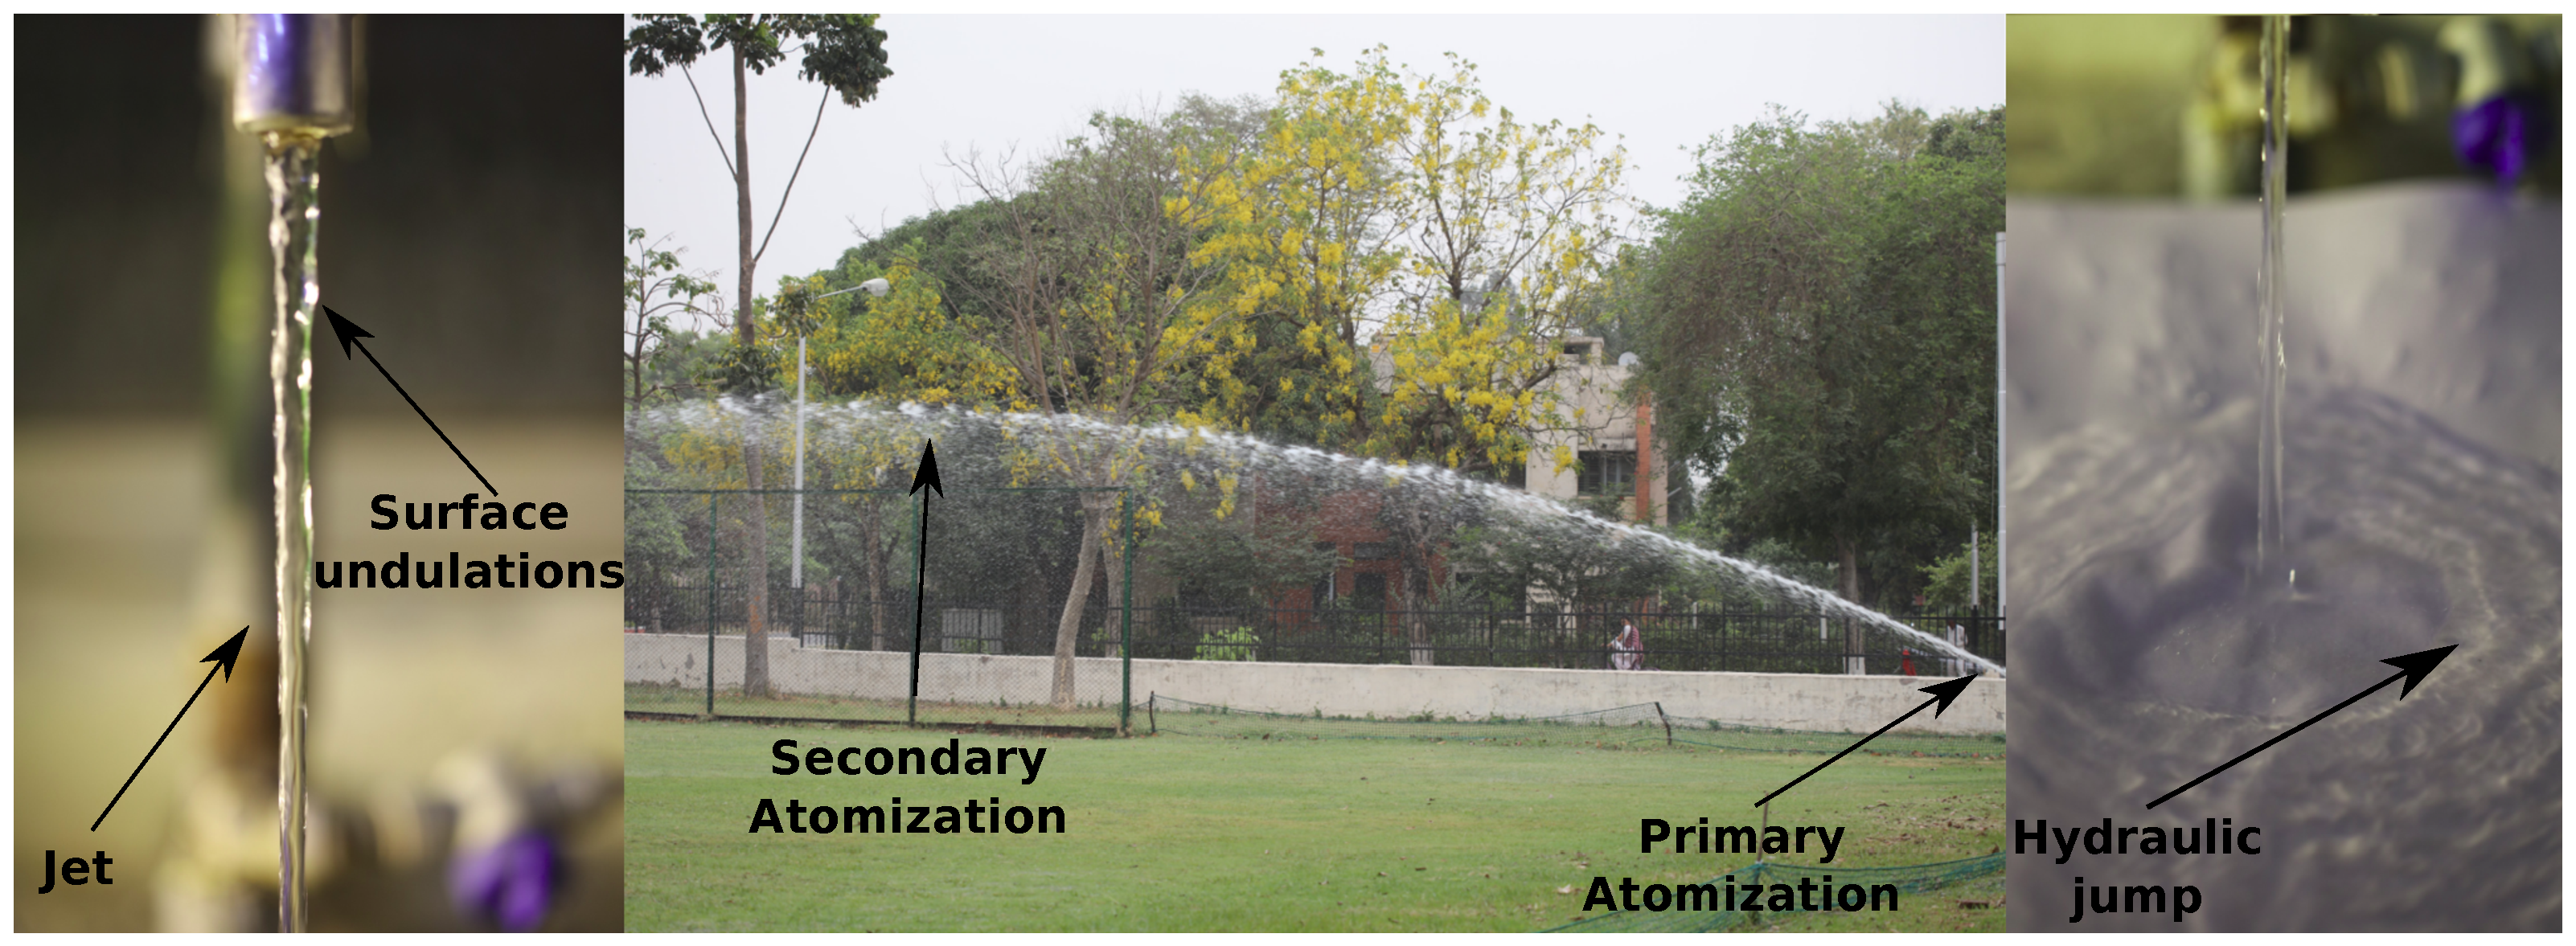
\includegraphics[width=\textwidth]{chapters/introduction/examples}
\caption{Liquid jets in everyday lives: (a) a typical jet with surface undulations, (b) liquid sprinkler showing different regimes of jet atomization, and (c) a jet of water falling onto a solid substrate.}
\label{Figure::examples}
\end{figure}
\subsection{Jet - solid interactions}
Figure~\ref{Figure::examples}(c) shows a liquid jet impingement onto a solid surface, and accompanying hydraulic jump. This configuration has several aesthetic and industrial consequences. One everyday example can be observed in the classically studied hydraulic jump in kitchen sink \citep{eggers2008physics}. With respect to industries, liquid jet impingement is used for achievement of high heat transfer coefficients for cooling of turbine blades, electronic equipment and pistons \citep{bergles1983boiling,chen2018numerical}, water jet machining, and metal processing. Recently, building on the innovative works of \citet{kate2007hydraulic}, \citet{singh2018computational} presented an extensive investigation of the accompanying hydraulic jump during such impingements. In case of a vertical impingement, the liquid sheet spreads radially, and symmetric jump is observed whereas, in case of an oblique impingement, the asymmetric jump can be obtained. The interplay between wall-adhered outward flow and back-flow from the downstream of the sheet determines the physics governing formation and stability of these hydraulic jumps.   
\subsection{Jet - jet interactions}\label{section::jetJet}
Most elemental among the interactions of liquid jets is the collision between two identical jets. This configuration is one of the canonical configurations for generation of liquid sheets \citep{wadhwa2013noncoalescence}. It gives way to atomized droplets in high inertial regime \citep{bremond2006atomization}. If the strengths of the two jets are identical, the liquid sheet is formed, as a planar one, in the median plane, ie., mid-way between the jets at the point of collision \citep{bush2004collision}. This configuration is usually employed in the afterburners of the aircraft or in the thrust engines used in rockets \citep{chen2013high} and has advantages over the conventional coaxial liquid-gas jet atomization technique because of the improved inertial driven destabilization and mixing between jets \citep{erni2013free}. Moreover, the droplets formed in this process come from the thin sheet, making the droplet size distribution skewed towards the lower size and more evenly spread \citep{inoue2008study,inoue2009liquid} as compared to the droplets formed from the single jet atomization as the latter are ejected from a thick liquid jet core instead of a thin sheet. This aids in the post-atomization combustion process \citep{lhuissier2011destabilization}. The collision of laminar jets to form stable sheets is the fundamental case of such atomization processes and also holds physical significance for the exploration of physics behind atomization. Moreover, these structures can be used as wall-free continuous reactors \citep{erni2013free} as well. Recently, \citet{koralek2018generation} demonstrated the generation of the free-flowing sheet with the thickness in the order of few nanometers. These sheets can be used for Infra-Red, X-ray and even electron spectroscopy.\\
\begin{figure}
\centering
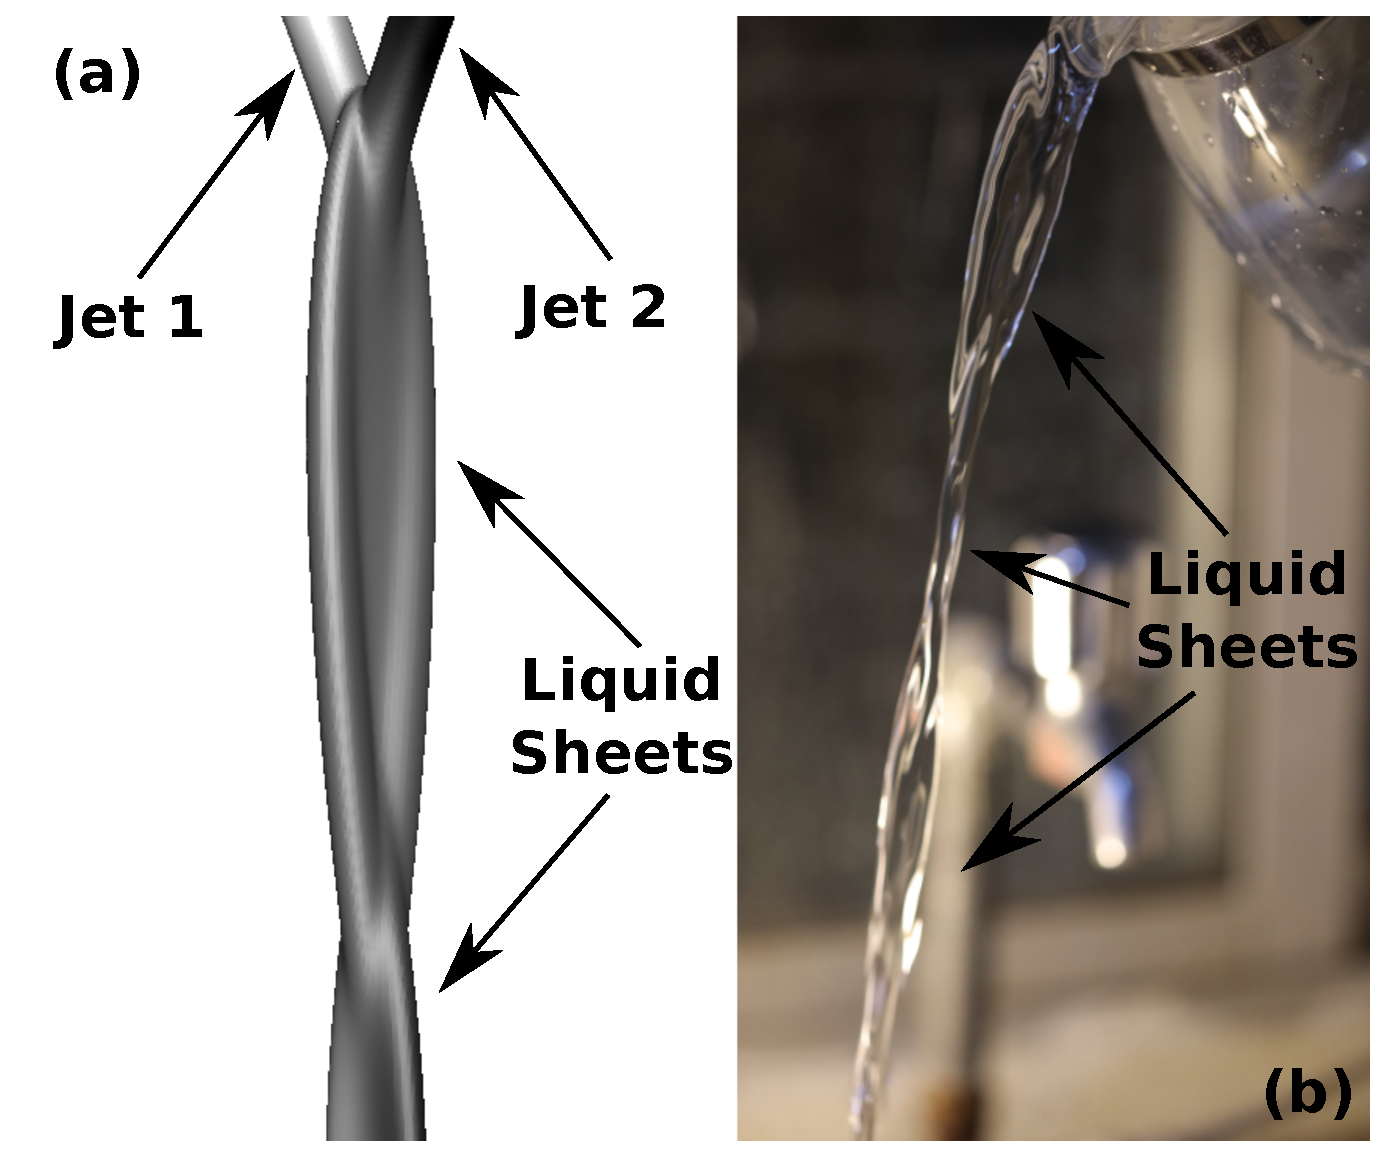
\includegraphics[width=0.6\textwidth]{chapters/introduction/LinkChain}
\caption{(a) The consequences of collision of two liquid jets: a schematic and (b) a typical life of smooth liquid jet, freely falling under the influence of gravity. Both these configurations result in the formation of the liquid chain structure.}
\label{Figure::JetJetSchematic}
\end{figure}
At low velocities or narrow angles of impingement, jets may coalesce to form a unified one or they may bounce off due to the presence of a thin film of air between them \citep{wadhwa2013noncoalescence}. On increasing the flow rates, laminar jets may lead to the formation of a stable liquid sheet bounded by the thicker rims at the periphery \citep{yang2014liquid}. The inertial and the gravitational forces act to expand the liquid sheet formed, but the action of surface tension helps the sheet to converge so that the successive collisions of the thick rims downstream of the flow result in the formation of mutually orthogonal liquid sheets \citep{bush2004collision}. Figure~\ref{Figure::JetJetSchematic}(a) illustrates this structure termed as the liquid chain with the complementary orthogonal sheets forming the different links. A similar structure can also be observed when a liquid sheet falls under the influence of gravity. The sheet has minimum thickness at the center, whereas at the periphery, by virtue of surface tension, thicker rims are present. These rims undergo collision to form subsequent sheets. A daily life example could be pouring out of water from jet as illustrated in Figure~\ref{Figure::JetJetSchematic}(b). It  must be noted that for these interactions, the liquid jet must be small enough to allow Rayleigh-Plateau instabilities to kick in \citep{eggers2008physics}.
\subsection{Jet - pool interactions}\label{section::jetPool}
\begin{figure}
\centering
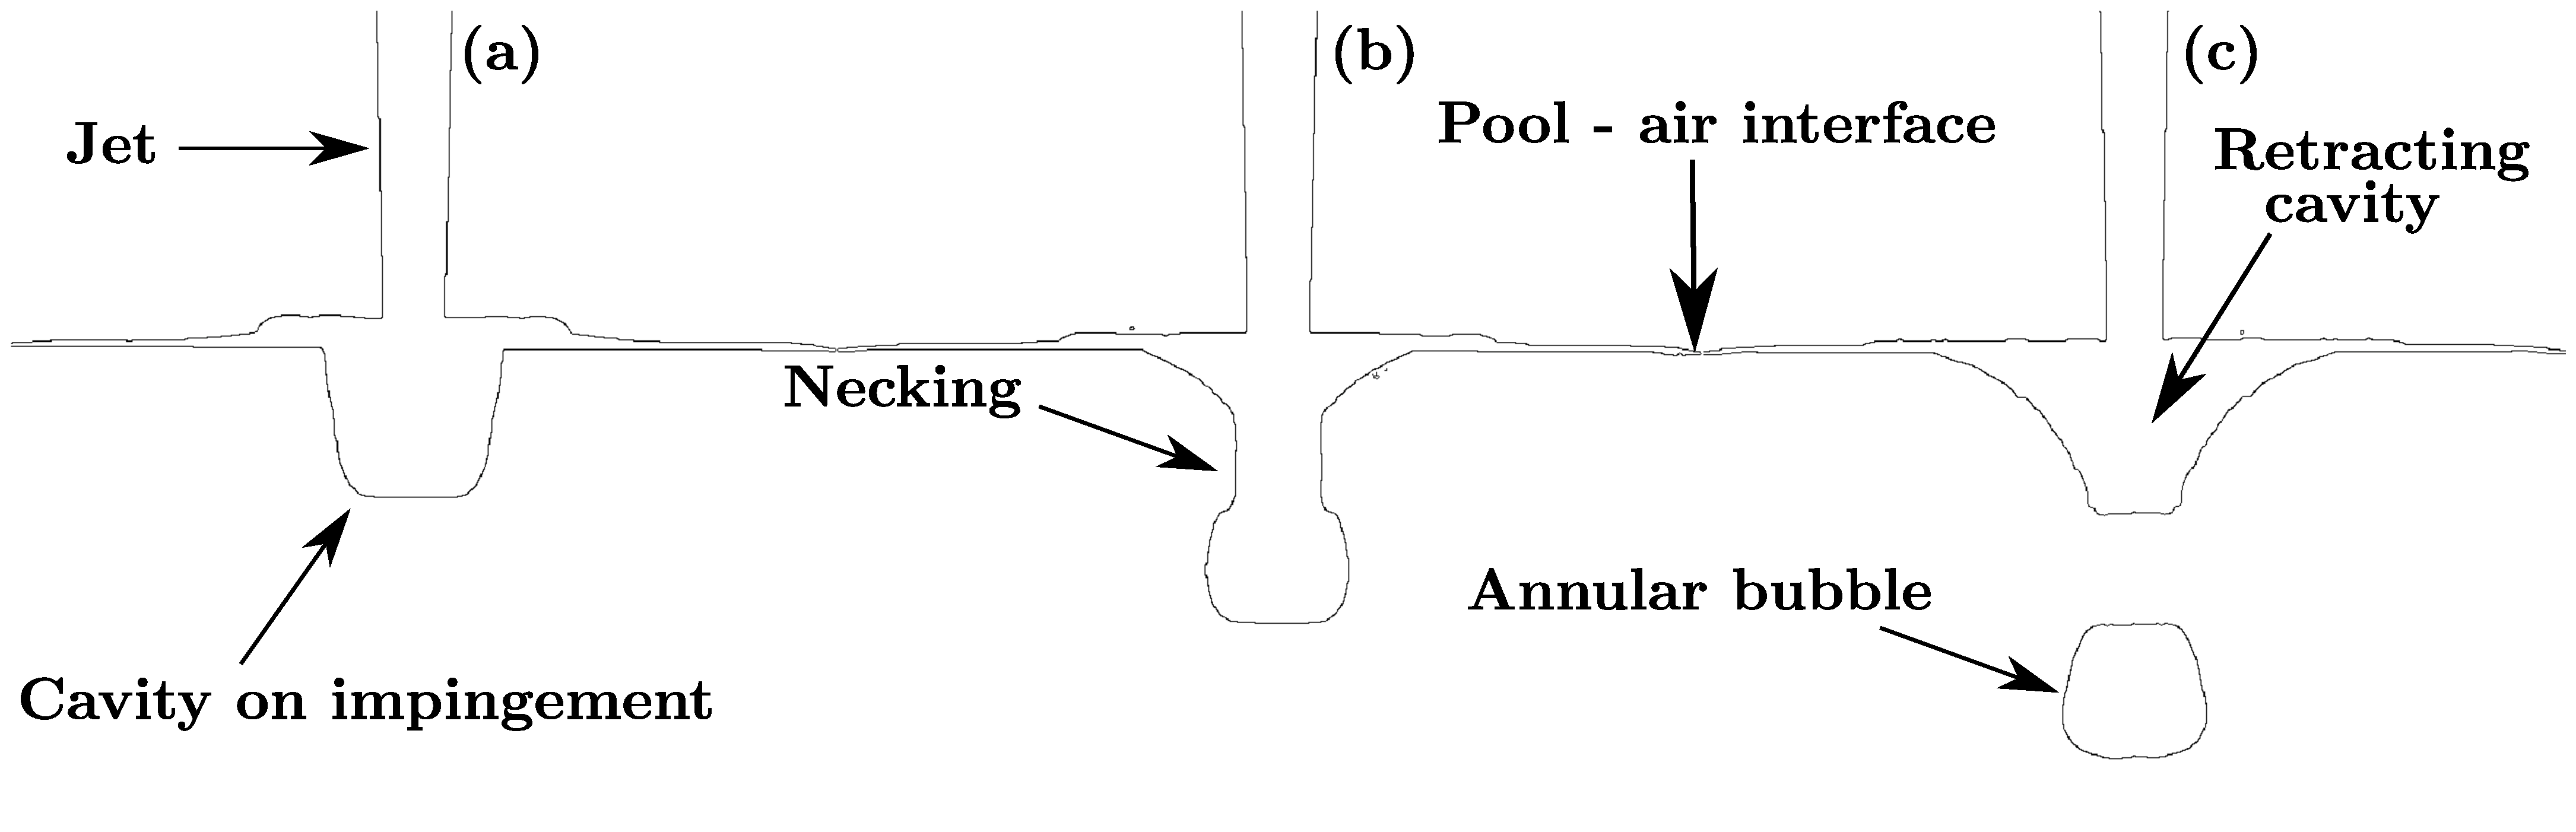
\includegraphics[width=\textwidth]{chapters/introduction/EntrainmentSchematic}
\caption{Illustration of the bubble entrainment by a single jet: (a) jet impingement and formation of cavity, (b) cavity growth and necking, and (c) pinch-off of first annular bubble and retracting cavity.}
\label{Figure::EntrainmentSchematic}
\end{figure}
Entrainment inside a pool, beneath a plunging liquid jet, plays a favorable role in aeration process of chemical reactors \citep{Bin1993}. A look around reveals the presence of this phenomenon in everyday life, ranging from filling of a glass of water using tap to several industrial processes. The plunging jet configuration is often used in wastewater treatment plants \citep{van1979effect} and have several other industrial applications, like gas-liquid mixing and reactions \citep{Mckeogh1981} and operation of jet propulsion vehicles (navy vessels) \citep{deshpande2012computational}. It can also be used in several oxygenation processes, especially in fish-keeping. However, the air bubbles can be detrimental in processes like casting, causing a reduction in strength of the resultant mold. It is of utmost importance to understand the process of entrainment before controlling it, either in favorable or opposing direction. The critical velocity of the liquid jet for the inception of entrainment depends on the dimensions of the jet \citep{lin1966gas,Chanson2004} and the disturbances present on its surface \citep{sene1988air}. Figure~\ref{Figure::EntrainmentSchematic} illustrates the process of air-entrainment initiation. Near inception, flow conditions have been revealed by \citet{Cummings1998,Cummings1999} as symmetric cylindrical air-entry about the centerline of the vertical jet \citep{Roy2013} (Figure~\ref{Figure::EntrainmentSchematic}(a)). Air entry as unified mass is restricted by surface tension causing pinch off of bubbles (Figure~\ref{Figure::EntrainmentSchematic}(b)). After the pinch-off occurs, the cavity retracts back to the pool surface and this cycle repeats for continued entrainment \citep{Roy2013} (Figure~\ref{Figure::EntrainmentSchematic}(c)). The continuous pinch-off pertains towards a statistically steady state and this bubble population behaves like a single cluster whose characteristics play a crucial role in two-phase chemical reactors \citep{Chanson1994,Clanet1997,Bagatur2014,Harby2014}. Some recent studies by \citet{ma2011comprehensive,ma2012two} have revealed the critical role of velocity gradient at the impinging interface. They have also analyzed the void fraction and bubble count inside the liquid pool. At very high inertia of liquid jets, the bubble cluster become chaotic. One such situation is depicted in Figure~\ref{Figure::entrainmentExample}.
\begin{figure}
\centering
\includegraphics[width=0.4\textwidth]{chapters/introduction/entrainment}
\caption{Entrainment inside a liquid pool. High inertia liquid jets lead to chaotic flow of entrained bubbles.}
\label{Figure::entrainmentExample}
\end{figure}
\section{Literature Survey}
In the present work, liquid jet interactions of types described in sections~\ref{section::jetJet} and~\ref{section::jetPool} are thoroughly investigated. Therefore, in this section, the literature pertaining to these two studies is discussed.
\subsection{Collision of liquid jets}
\citet{rayleigh1879capillary,rayleigh1889tension} was probably the first researcher to formally study the chain-like structures. He reported that the chain structure was generated because of the undulations formed at the surface of a single elliptical liquid jet. Unlike cylindrical jets, they do not have an axis of overall symmetry. This results in thickening of the jet at the periphery (similar to Figure~\ref{Figure::JetJetSchematic}(b)) leading to the formation of the chain-like structure due to the impact of these rims.\\
\citet{taylor1960formation} formulated an impingement theory for impact of liquid jets to form a fluid sheet at the median plane, mid-way between the jets. Prior to his work, only the inertial and gravitational forces were considered to describe the phenomenon which gave an expanding liquid sheet. He realized that the flow inside the thicker rim at the periphery can be sustained only if the  surface tension force provides the necessary centripetal acceleration to the fluid parcels inside the rim. The velocity field in the rim is also accelerating due to loss of gravitational potential. On balancing the inertial and surface tension forces, \citet{taylor1960formation} proposed an expression for the sheet radius, given by $r_{max} = \rho u_0Q(\theta)/(2\sigma)$ (where, $u_0$ denotes the average sheet velocity assumed constant throughout including the rim, $Q(\theta)$ implies liquid flux distribution inside the sheet and $\rho$, $\sigma$ are the fluid density and its surface tension coefficient with the air, respectively).\\
\citet{ibrahim1991impinging} demonstrated that the stable sheet structures can serve as the base case for the atomization studies because the droplets are formed from the perturbed liquid sheet. At high viscosities, different flow instabilities die down but at higher inertial strengths, as the flow becomes turbulent, the flapping atomization takes place.\\
\citet{clanet2002life,villermaux2002life} discussed the instabilities inside the liquid sheet. As the velocity exceeds a critical value, the Kelvin-Helmholtz instability takes over and results in formation of destabilizing waves. This also speeds up the process of fingering instabilities at the peripheral rim of the sheet.\\
\citet{bush2004collision} worked on the classical formulation proposed by \citet{taylor1960formation} and gave a comprehensive theoretical and experimental theory for collision of liquid jets. They introduced several regimes to characterize the different flow structures obtained from such collisions and gave an exhaustive experimental analysis of the stable liquid chain formed by the collision of laminar jets. Their work also verifies the formulation given by \citet{taylor1960formation} which predicts the sheet dimensions within experimental precision. Emphasis has been also given by \citet{bush2004collision} for prediction of shapes of leaf-like links forming chain structure. We have used the results developed by them to validate our numerical model.\\
\citet{bremond2006atomization} studied the several instability modes related to the rim at the periphery of the sheet. These instabilities are magnified as the velocity of fluid parcels inside the rims increase and the curvature dependent surface tension forces are not able to maintain equilibrium. First, finger-like projections are observed at the rims' outer boundaries causing Plateau-Rayleigh instability and droplet generation.\\
\citet{choo2001parametric,choo2002velocity,choo2007effect} have worked extensively on the characterization of the first link of the chain structure, including the velocity field inside. Contrary to the earlier belief, they have shown that the sheet velocity is not a constant parameter but varies with the azimuthal angle variation. This has been demonstrated in our studies as well. Moreover, they have also discussed the variation in the sheet characteristics with respect to the velocity profile at the exit of the nozzles, inside the jets. They prescribe that a parabolic profile gives a better estimate for the fully developed laminar jet as compared to the uniform profile or any other power law fit. Further, they gave the justification for the presence of thicker liquid rim at the periphery using Particle Image Velocimetry (PIV) technique. The radial streamlines were observed near the point of impingement and the fluid parcels travel towards the periphery resulting in the formation of the thick rim due to fluid accumulation. \\
\citet{chen2013high} have shown the formation of liquid chain using Finite Volume based Volume of Fluid (VOF) framework. They attempted the reproduction of different flow regimes as proposed by \citet{bush2004collision}. The same numerical framework is used in the present method with some modifications on the mesh refinement criteria.\\
\citet{inamura2014effect} studied the presence of stagnation point inside the liquid sheet. Unlike the head-on collision of liquid jets where this point is at the intersection of the jets, it was found to shift upstream by some factor. The factor was found to be dependent on the impingement angle. These works summarize the variation of fluid velocity inside the sheet.\\
\citet{yang2014liquid} discussed the influence of different flow parameters on the shape and size of the first link in the chain structure. They acknowledged the variations due to physical parameters as well. In the present study, their arguments are generalized for the entire chain structure.\\
\citet{da2016surface} also demonstrated the formation of liquid chain using Boundary Element Method (BEM). This simulation work comprises of inviscid flow assumption but gives mesmerizing fluid structures. They have successfully reproduced all the regimes observed in the experimental works but fail to acknowledge the internal dynamics of the liquid sheet.
\subsection{Air entrainment by impingement of liquid jet on a pool}
\subsubsection{Experimental work}
\citet{Bin1993} gave an extensive review of all the theoretical and experimental work present at that time. The compiled works include description of entrainment mechanism, conditions for its onset, details of entrained cluster and empirical formulas for associated mass transfer. The review paper also consisted a detailed description of two-dimensional jet impingement \citep{sene1988air, Goldring1980}.\\
\citet{Evans1996} identified that the gas entrainment rate depends on the effective diameter of the free jet at the plunge point and the annular film thickness adjacent to the surface of the jet. The works of \citet{Mckeogh1981,Van1981,el2002} recorded the air concentration profiles and velocity distribution in the fully developed flows. The authors targeted the global measurements of air entrainment.\\
\citet{Chanson1996} explained the mechanism of air entrainment with the help of an advection-diffusion model, resulting in a diverging entrainment cone. The region of pool surrounding the intersection of jet and pool acts as the source of bubble inception. Inside the pool, as the buoyancy balances the downward flow of bubbles, they start moving upwards. Depending on the inertia of incoming jet, either a converging-diverging or a diverging overall cluster is formed.\\
\citet{Clanet1997} reported some experiments conducted with round plunging jets that reveal interesting results concerning the depth of penetration of the bubble cluster under a wide range of jet diameters, velocities and plunging angles.\\
\citet{Cummings1999} studied extensively the effects of velocity on the air entrainment phenomenon and its quantity along with coalescence and breaking of individual bubbles.\\
\citet{Chanson2004} investigated air entrainment and bubble dispersion in the developing vertical circular plunging jets and came up with some remarkable results and expressed a requirement to study the air-water velocity distribution and turbulent velocity fluctuations.\\
\citet{Soh2005} gave an analytical approach to the problem. They have related the maximum height of the air void with the properties of water jet using the energy balance method. However, the method is too idealized, neglecting the losses and simplification of geometry. The theory seems to be in good agreement with the experimental results only for low diametrical Froude numbers ($ Fr_D < 10 $, where, $Fr_D = \frac{V_j}{\sqrt{gd_j}}$) with an error as high as 50\% for $ Fr_D > 50 $.\\
Efforts are also being noticed to understand the physics of entrainment using numerical approach. \citet{Qu2011} published a combined experimental and numerical investigation. They studied the mixture approach against the level-set method for flow modeling. Since, this phenomenon rigorously involves the consideration of interface and its deformations with time, level-set approach has an edge over the mixture approach.
\subsubsection{Numerical work}
\citet{Zhu2000} studied the mechanism of air entrainment due to surface roughness. However, the work involves numerical simulations only up to the impact and pinch off point. Recent study complies with the proposed air cavity formation reported in the above paper.\\
\citet{Kersten2003} examined the spread of falling liquid over the receiving pool, formation of cavity and eventual pinch off. The initial bubble that pinches off after the closure of cavity and the air sheathe around the submerged jet can be designated as the source of bubbles inside the pool. Recently, comprehensive research has been carried out on further characterization of different parameters related to entrainment \citep{Belden2012,Harby2014,Bagatur2014}. Several researchers have mentioned the requirement for the study of influence of the controlling parameters, such as jet length and the velocity on penetration depth and entrainment volume \citep{Qu2013}. \citet{Roy2013} examined descriptively the trajectory of a single bubble in the entrainment region.\\
\citet{Durve2012} outlined the onset of gas entrainment through numerical simulations. It can be easily established that over the past couple of decades, the main focus has been to explore the mechanism of the entrainment process.\\
\citet{kiger2012air} highlighted the role of air-entrainment for two distinct systems. The first included a standard configuration of single liquid jet impinged onto a stationary pool, and the other comprised on plunging horizontal waves. In an extensive review of available literature, the authors have investigated the flow inception conditions and given insights into the more complex, breaking wave entrainment. The surface vortices have been found to be an important aspect in this regard.
\citet{Deshpande2013} studied the distinguishing features of the shallow angle plunging jets using VOF methodology. However, the work deals with inclined jets and till the pinch off moment for vertical jets.\\
\citet{Brouilliot2013} reported remarkable compliance of numerical and experimental results with classical VOF-PLIC method. At the same time limitations of this method to account for inclusions smaller than the mesh grid size can be observed.\\
\section{Lacuna in literature}
\subsection{Collision of liquid jets}
Critical assessment of literature reveals that an in-depth study of fluid chain regime is still due which can explore fundamental physics behind the formation of primary link and establish a relation between successive diminishing links. Moreover, most of the analytical or empirical models, used to describe the flow, need input from the experiments to close the system of equations prior to obtaining any solution \citep{bush2004collision}. The work in the direction of numerical simulation to obtain such structures is few as per the knowledge of the author \citep{chen2013high,da2016surface}. A major challenge that lies in the prediction of the chain-like structure is the proper resolution of the sheet (approximately $1/100^{th}$ of jet diameter) between the rims, which are supposed to mingle once again for forming next link in a mutually perpendicular plane. \citet{chen2013high} have demonstrated the presence of a diversity of length scales in such a simplistic fluid link. If the grid resolution is not sufficient, occurrence of numerical pinch-off is observed, whereby non-physical holes are created inside the sheet because of the lack of cells. The works of \citet{da2016surface} do give satisfactorily result in this regard but, their exhibition of chain-like structure along with other physical jet related structures is limited to inviscid fluids. The inability of their numerical model to incorporate viscosity has led to inaccuracies in the study of chain structure along with its kinematics and dynamics.
\subsection{Air entrainment by impingement of liquid jet on a pool}
Most of the theoretical works prior to the review by \citet{Bin1993} included two-dimensional plunging liquid jet. However, from an industrial point of view, three dimensional jets are more important since they are easy to achieve and widely studied by researchers. Nevertheless, there have been only a few studies on the flow fields just below the impingements. Most of the works revolve around what \citet{Bonetto1993} termed as the global measurements. Undoubtedly these studies are important to have a control over the process and may allow correlation of the onset of air-carry under criteria. However, very little or no information is provided about the kinematics and dynamics of the entrained bubbles and the resultant dispersion of the submerged jet. Even though this process is so common in nature, the mechanism involved is not well understood. Entrainment characteristics need to be related with flow rate, jet diameter and length of jet for better understanding. Irrespective of such attempts at development of correlations, as argued by \citet{Van1976}, a lack of generality is observed (discrepancies of the order of 3 or more). It has been observed that the parameters proposed by one investigator is off by noticeable amount when compared to data from others. Furthermore, the literature still lacks an exhaustive account for the analysis of bubble life cycle during entrainment. Moreover, there have been very little work on the characterization of the region affected in the liquid.
\section{Objectives of the present work}
\subsection{Collision of liquid jets}
\begin{enumerate}
\item [$\bullet$] To understand the formation of fluid chain through a series of temporal snapshots leading to the formation of a steady structure after initial transients.
\item [$\bullet$] To study the overall behavior of the fluid chain while focusing on the physics of flow for the primary link by analyzing the dimensional characteristics and velocity fields.
\item [$\bullet$] To generalize the overall behavior of the fluid chain structure from the characteristics of the first link.
\item [$\bullet$] To model the collision of liquid jets in a manner analogous to the impact of discreet non-deformable fluid parcels (hereinafter referred as fluid quanta or particles). 
\item [$\bullet$] To analyze the formation of higher order links as a result of the collision of rims of the preceding links. 
\end{enumerate}
\subsection{Air entrainment by impingement of liquid jet on a pool}
\begin{enumerate}
\item [$\bullet$] To understand the formation of air cavity and subsequent pinch off details along with fragmentation of the initial bubble into smaller bubbles.
\item [$\bullet$] To characterize the cluster of bubbles and the region of entrainment in the liquid pool. 
\item [$\bullet$] To study dynamic behavior of the interface cluster and observe the variation in shape with time starting from the point of inception of entrainment.
\item [$\bullet$] To investigate the kinematics and dynamics of bubble lifecycle, commencing at the time of entrainment to its trajectory inside and outside the bubble cluster to the instance when it erupts at the water surface.
\item [$\bullet$] To develop a conductivity probe in order to obtain strength of entrainment at different flow rates.
\end{enumerate}
\section{Organization of the thesis}
The current work is undertaken to understand the fundamental physics behind two important jet interactions categories, namely, collision of liquid jets to form chain and impingement of jet onto a pool to initiate entrainment. The present chapter summarizes the work available in the literature, and the scope of improvement. The following chapter includes the description of the mathematical model, as both the topics involve detailed numerical simulations. Chapter~\ref{Chapter::jetJet} represents the results corresponding to the collision of laminar smooth liquid jets. At first, a series of transient features are studied to reach a steady state structure. We have  Special attention is given to the second and third collisions, leading to the formation of the subsequent mutually orthogonal links. The flow kinematics are studied based on the velocity field inside the sheet. The impact of fluid quanta is then used to model the behavior of fluid parcels inside the sheet. Post-collision, the effect of surface and viscous forces is included with a constant magnitude force, which is always perpendicular to the trajectory of individual fluid quantum. This helps to understand the dynamics of liquid sheet formation. The second important aspect of our work is to generalize the impingement model for the entire chain structure, taking into account the reduced strength of rims that collide to form the subsequent perpendicular links.\\
Furthermore, chapter~\ref{Chapter::BubbleEntrainment} consists of the results for impingement of liquid jet onto a pool surface. It is a combined experimental and numerical study to understand the process of entrainment inception and subsequent cluster formation. Different modes of entrainment are discussed followed by study of the onset of entrainment. The life cycle of first annular bubble, from the time of inception, is investigated in detail. Furthermore, the association of air bubbles formed by the fragmentation of first annular bubble and continued entrainment results in formation of a cluster. This has been treated as an individual system, and different kinematic and dynamic features are discussed. At last, a conductivity probe is used to investigate the bubble kinematics.
